% Requirements:
% Minimum 5 pages.
% single-column, Times New Roman, Font 10, 1 inch margins all around.
\documentclass[conference, 10pt, onecolumn, draftclsnofoot]{IEEEtran}
% Standard packages
\usepackage{cite}
\usepackage{amsmath,amssymb,amsfonts}
\usepackage{algorithmic}
\usepackage{graphicx}
\usepackage{textcomp}
\usepackage{xcolor}
% For hyperlinks
\usepackage{hyperref}
% For Times New Roman
\usepackage{mathptmx}
% Subfigure captions
\usepackage{subcaption}
% SVG graphics support
\usepackage{svg}

\def\BibTeX{{\rm B\kern-.05em{\sc i\kern-.025em b}\kern-.08em
    T\kern-.1667em\lower.7ex\hbox{E}\kern-.125emX}}
\begin{document}

\title{Input-Based HPC Run Time Prediction}

\author{\IEEEauthorblockN{Kenneth Lamar}
\IEEEauthorblockA{\textit{Department of Computer Science} \\
\textit{University of Central Florida}\\
Orlando, United States \\
kenneth@knights.ucf.edu}}

\maketitle

\begin{abstract}
Predicting the run time of an application is difficult for humans.
Sometimes, it is difficult to understand the relationship between the adjustment of an input parameter and its resulting effect on run time.
Other times, users simply want to run their job and do not care enough to provide an accurate run time estimate.
In high performance computing (HPC), poor predictions result in suboptimal scheduling, or worse, job termination before application completion.
In this work, we present a machine learning model to predict the run time of applications accurately and automatically, novelly using the job inputs as predictive parameters.
We propose the use of the random forest regressor, which was found to perform best on average among 180 model variants ran on three proxy apps.
Ultimately, we found that random forest regression consistently offered state-of-the-art accuracy, as high as 99\% and always competitive.
\end{abstract}

\begin{IEEEkeywords}
run time prediction, machine learning, high performance computing
\end{IEEEkeywords}

\section{Introduction}
% background, problem, importance, existing literature, system overview, data collection, components of your ML system, experimental results

% Background
High performance computing (HPC) is used to solve problems that would be impossibly large on conventional machines.
HPC platforms consist of many server-grade machines linked via a high-performance network interconnect, working on large, distributed problems.
To manage these resources between tasks, a job management system, such as SLURM~\cite{SLURM}, is used to schedule jobs.
Scheduling behavior is based on expected resource usage, such as node count and run time.
Providing accurate predictions improves scheduling quality.

% Problem, Importance
Jobs in SLURM are provided in the form of a submission script.
To provide expected resource usage to SLURM, users must specify the expected run time of the job in its submission script.
If the user overpredicts the run time, it will result in wasteful scheduling, as the scheduler will have already made scheduling decisions under the assumption that the job needed more time. 
If the user underpredicts, then the job will be terminated early.
This happens because the expected run time is typically used in scheduling as the upper bound on the job's allowed run time.
Thus, accurate predictions are necessary in HPC to improve scheduling quality.

% Existing literature
In the user-led approach, users are often bad at predicting job run time.
Typically, users do not want to take the time to determine an accurate run time prediction, even if they are skilled enough to do so, as this takes away time from the work they are trying to perform on the cluster.
Even when they do have an accurate run time, they are incentivized to overpredict, to prevent jobs from being killed early.

An alternative is a machine-based predictor.
Machines often make their predictions based on historic data.
They typically consider only data common to all jobs at their start, such as job name, username, user-provided run time prediction, and number of requested nodes.
This data has been applied both to traditional algorithms as well as machine learning approaches.
This approach has significant limitations; it misses the underlying inputs used by the job, which often have dramatic impacts on total job run time.

% system overview
In this work, we propose a machine learning pipeline that predicts the run time of applications using application-specific input parameters as training data.
%data collection
Data was collected on Voltrino, an HPC testbed.
We ran synthetic tests with randomized parameters on three proxy apps, ExaMiniMD~\cite{ExaMiniMD}, SWFFT~\cite{SWFFT}, and NEKbone~\cite{NEKbone}.
% components of your ML system
We removed unchanging parameters, then fed the training data into a random forest regressor model.
% experimental results
When testing with five-fold cross-validation, our model performed well against the baselines in all proxy app scenarios, always providing at least a top 10 result against 180 model variants and often providing the best results across all models.

\section{Important Definitions and Problem Statement}

\subsection{Important Definitions}

% Data
Our data consists of job input parameters, the data passed into an application, either from file or from command line arguments.
The core intuition is that these parameters are principally responsible for changes to job run time.
Parameters include both discrete named data (ex. the name of an execution mode) as well as various numeric types (ex. float, int), depending on the test.
We also recorded the node and task count for each job, as this determines how many resources are allocated to each job.
Whether or not the job crashed is also provided in the training data.

% Prediction target
Our prediction target is job run time.
As run time is a continuous value, our task is a regression problem.
Each job run time in seconds is recorded in the output of each test performed and linked to its associated job input parameters for use in the training and testing data sets.

% Variables or concepts in your data
All data in our data set is clean and precise data that directly corresponds to job run time.
The only uncertainty present in the data is run time variance from external factors, such as network congestion.
However, discussions with our Sandia partners suggest that the Voltrino network interconnect is hard to saturate, and thus run times should be relatively unaffected by external factors on this test bed.

\subsection{Problem Statement}
% Problem Statement:
%     Given: What is the problem. What is provided?
%     Objective: What is the goal?
%     Constraints: Any constraints, if present.

% Given
For this machine learning project, we want to accurately predict job run times.
We are provided a set of job input parameters associated with each run, and the resulting run times corresponding to each test.
% Objective
The objective is to learn the function that relates app input parameters to run times, a regression task.
% Constraints
% None really.

\section{Overview of Proposed Approach}

In this work, we propose the use of input parameters for use as machine learning parameters to predict job run time.
Traditional approaches use only on data that is standard to all jobs: job name, username, user-provided run time prediction, number of requested nodes, etc.
While the traditional approach is applicable to any job submitted to the SLURM scheduler, it can provide only a rough approximation of run times.
These approaches tend to rely on other factors, such as recency, predicting that jobs will take a similar amount of time as recent jobs with similar parameters did.
This is typically a reasonable assumption, for instance, when a user keeps running the same job with minor tweaks, but it makes the predictor incapable of predicting major changes because the underlying job inputs are opaque to the predictor.
In contrast, job input parameters can capture information that can apply to jobs that have never happened before, without the reliance on recency.
Machine learning provides the generality to train to each job and learn the significance of each input parameter on final run time, as well as their interrelationships.

In this work, all aspects of the machine learning pipeline were handled using the scikit-learn~\cite{scikit} framework.
At a broad level, our proposed machine learning pipeline uses the random forest regressor with 100 fully expanded trees, requiring minimal pre-processing.
Existing works have found random forests to offer state-of-the-art results as well as short training times~\cite{survey,7776517,PRIONN,10.1007/978-3-030-48340-1_48}.

\section{Technical Details of Proposed Approach}

% How features are extracted
Features are extracted using a testing script that saves randomly generated valid input parameter sweeps to a CSV file alongside the job run time.
All input parameters have the potential to be important to the training data, and thus all are initially provided to the model.
% Filtering
From there, if a parameter is left unchanged in all tests associated with a particular proxy app, it is filtered out.

% Pre-processing
For pre-processing, all non-numeric features are converted to numeric equivalents using a label encoder.
This is required because all training features must ultimately be provided to the model as floating-point numbers for scikit-learn.
Finally, all features are standardized, as this was found to improve prediction accuracy for nearly every tested model.

% Proposed model
We propose the random forest regression model.
Existing work has found that this approach provides the best results~\cite{survey,7776517,PRIONN,10.1007/978-3-030-48340-1_48}.
% Parameters
Random forests are valued for their flexibility, requiring minimal pre-processing to get a good result.
As a result, little tuning was required.
We set our forest size to 100 trees.
Each tree was set up to grow fully, with no impurity threshold or depth limits.
% Brief discussion of math if you want
% Not worth adding at this time.

\section{Experimental Results}

% Data description
\subsection{Data Description}
The data set consists of numerous runs of three proxy apps representative of common HPC workloads, ExaMinMD, SWFFT, and NEKbone.
This data set was generated on Voltrino, a 24 node Knights Landing (KNL) cluster at Sandia National Labs.
Voltrino is a testbed based on the Cray XC40 design used in the Trinity cluster\cite{Trinity}.
Runs were synthetically generated and tested using parameters randomly chosen between sane input ranges.
The number of nodes was varied from 1 to 4 and the number of tasks was varied from 1 to 32 to evaluate the impact of adjusting the number of available resources on run times.

ExaMiniMD~\cite{ExaMiniMD} is a modular application used in the simulation of molecular dynamics.
This application's input is contained entirely within an input file.
Valid input files are LAMMPS~\cite{LAAMPS} input scripts, with a subset of supported operations.
Tests on this proxy app consisted of two major use cases, a SNAP simulation and a 3D Lennard-Jones melt.
Within both cases, the lattice size, time step size, and number of steps was varied at random for each test.
Our final ExaMiniMD data set comprised 1,562 test runs and 21 features.

SWFFT~\cite{SWFFT} is a standalone version of the distributed 3D Fast Fourier Transform (FFT) application used by HACC.
Application input parameters for this app consist entirely of command line arguments.
All available parameters were adjusted, including the grid size on each axis (X, Y, and Z) and the number of repetitions.
Our final SWFFT data set comprised 1,618 test runs and 7 features.

NEKbone~\cite{NEKbone} is a Helmholtz equation solver for physics calculations, pared down from functionality in Nek5000 software.
All available parameters were varied between sane defaults.
Input parameters were passed in via an input file.
Unlike the other proxy apps tested, NEKbone was constrained to test only on one node with 10 tasks, as the version used was compiled to run on exactly 10 machine cores.
Our final NEKbone data set comprised 1,579 test runs and 12 features.

% Evaluation metrics
\subsection{Evaluation Metrics}
Prediction quality was measured using five-fold cross-validation of the correlation coefficient, $R^2$, as well as the root-mean-square error (RMSE).
$R^2$ is a standard way to measure prediction accuracy in regression tasks.
With this metric, an $R^2$ of 1 is perfect correlation between the predicted and actual run time, 0 means the predictions are of equivalent quality to always predicting the average run time, and negative values of $R^2$ are for anything worse than that average.
$R^2$ results are reported in \figurename~\ref{fig:R2}.
RMSE reports the square root of the sum of the squares of each feature error.
It is a standard risk metric used to report loss.
RMSE results are reported in \figurename~\ref{fig:RMSE}.
For all metrics, five-fold cross-validation is used as an easy way to split the training data from the testing data, with the average of those runs reported in the results.

% Baseline methods for comparison
\subsection{Baseline Models}
We compared our proposed model against seven alternatives, varying major model parameters to tune for best results.
We also tried each model against three slightly adjusted pre-processing techniques, since some models benefit from adjustments to the input data set.
This resulted in a total of 180 model variants, with each of these variants tested against our three proxy apps.

As baselines, we compared against the Bayesian ridge regressor, the linear stochastic gradient descent (SGD) regressor, and the decision tree regressor, all with default parameters in scikit-learn.
We also compared against the support vector regressor with RBF; sigmoid; and first, second, and third degree polynomial kernels.
We tested the k-nn regressor with k varied from 1 to 7.
We tested PLS regression, varying the number of components to keep from 1 to 4.
Finally, we tested against a variety of multi-layer perceptron (MLP) approaches, varying from 1 to 10 layers, with 100 hidden neurons per layer.
We evaluated several MLP perceptron types, including linear no-op (identity), logistic sigmoid (logistic), hyperbolic tangent (tanh), and the rectified linear unit (relu) perceptron functions.
All MLP approaches used the "adam" solver, a stochastic gradient-based optimizer.
Alternative solvers were attempted but offered poor results.

\subsection{Performance Results}
% Overall performance comparisons. Plots, descriptions of results, insights, findings from observations.

\begin{figure}
    \centering
    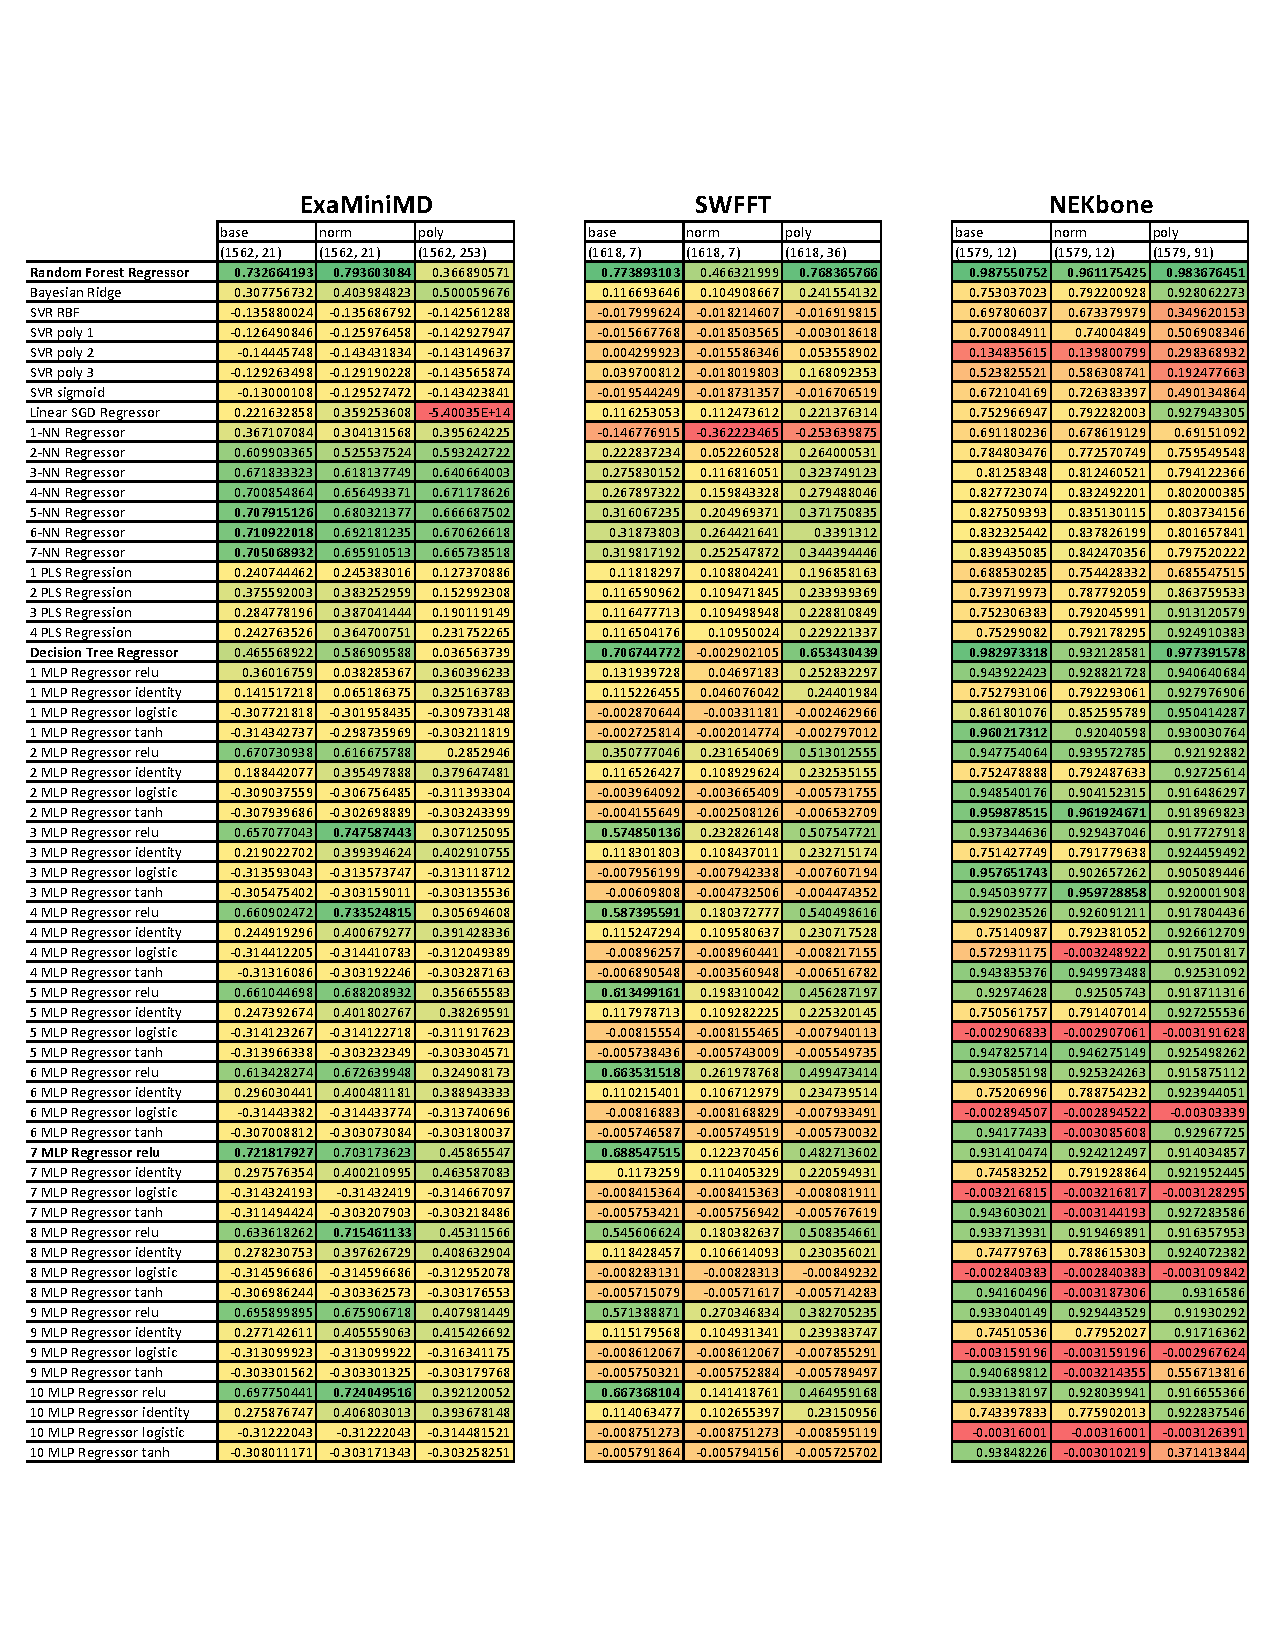
\includegraphics[width=\columnwidth]{Figures/R2.pdf}
    \caption{$R^2$ for each test. Color scales are used, where green indicates a good result, red indicates a poor result, and yellow indicates an average result. The top 10 best results for each proxy app are highlighted in \textbf{bold}.}
    \label{fig:R2}
\end{figure}

\begin{figure}
    \centering
    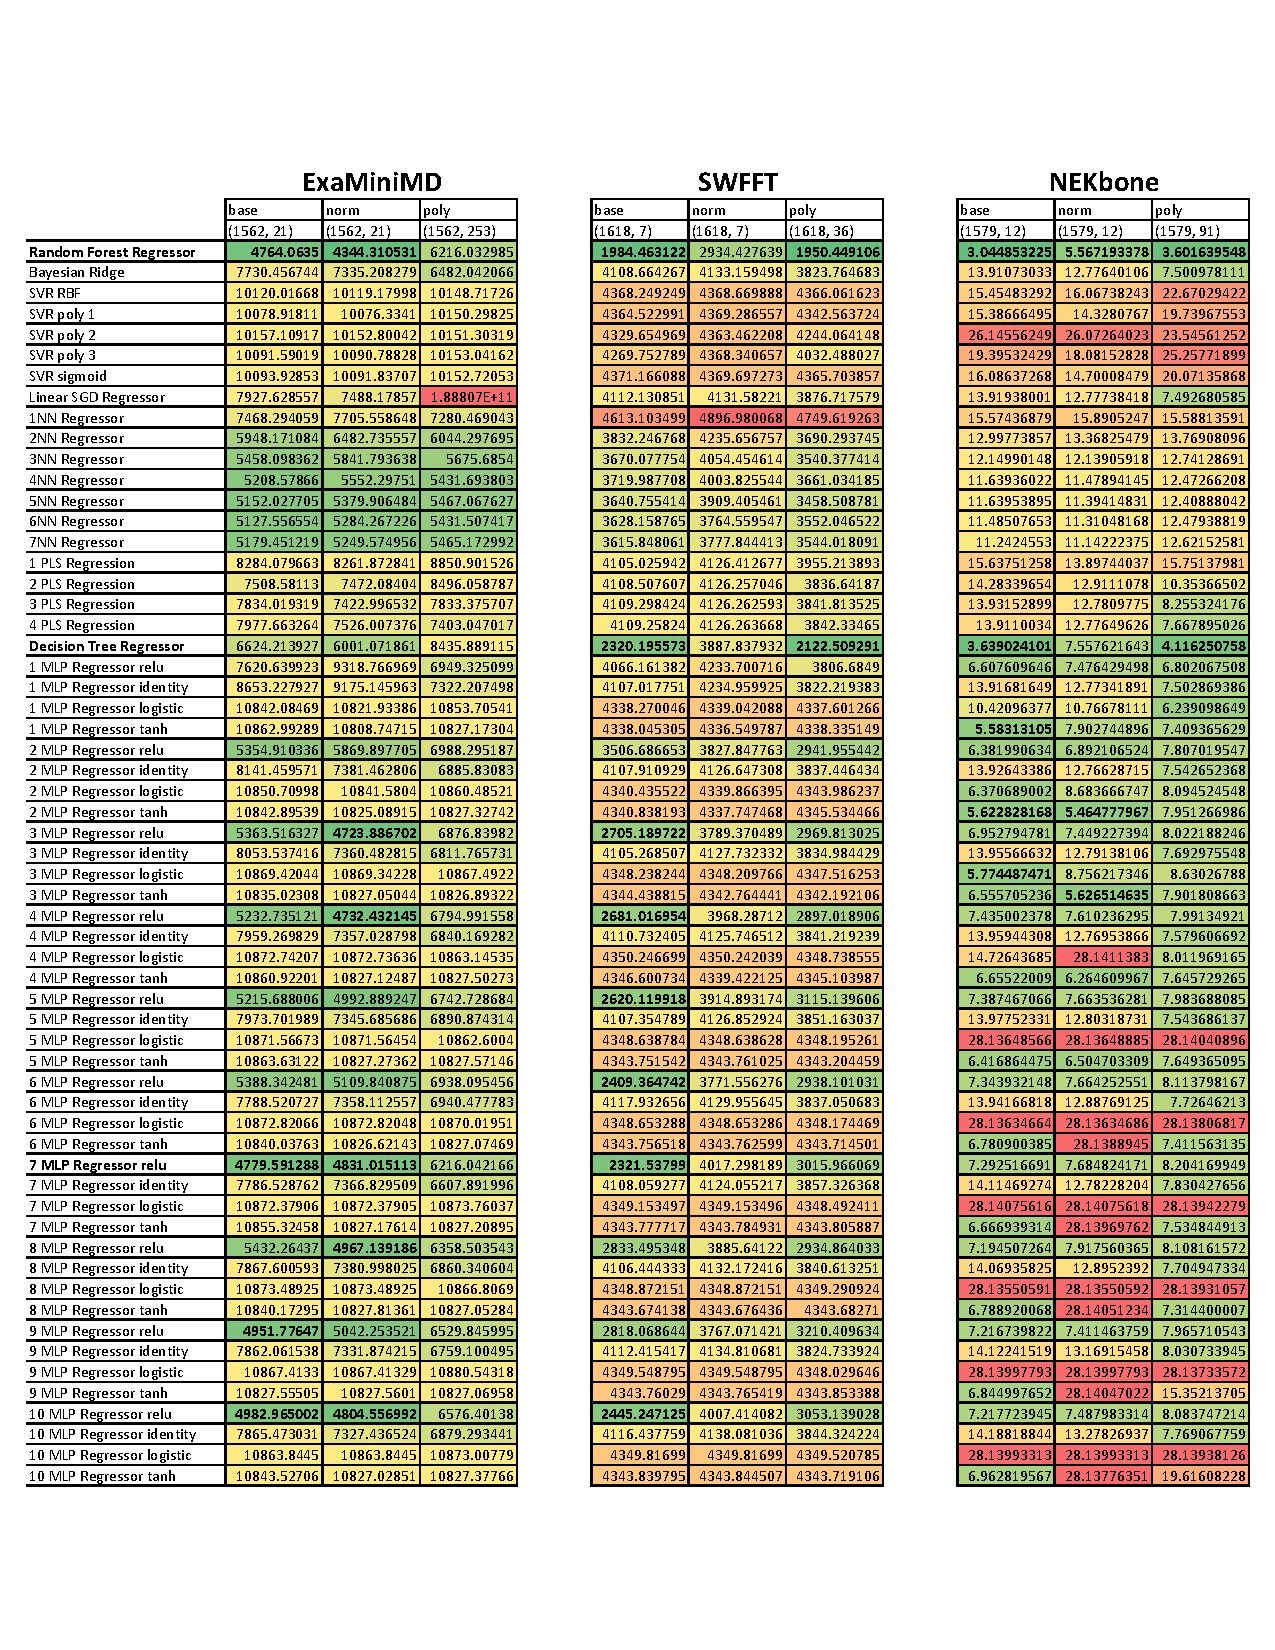
\includegraphics[width=\columnwidth]{Figures/RMSE.pdf}
    \caption{RMSE for each test. Color scales are used, where green indicates a good result, red indicates a poor result, and yellow indicates an average result. The top 10 best results for each proxy app are highlighted in \textbf{bold}.}
    \label{fig:RMSE}
\end{figure}

Full performance results are reported in \figurename~\ref{fig:R2} and \figurename~\ref{fig:RMSE}.
%The full raw performance results, data set, and scripts are available in the project GitHub repo at \url{https://github.com/KennethLamar/CAP5610/tree/main/Project/Final}.
In both figures, rows contain unique model variants and columns contain unique pre-processing variants.
Below each pre-processing variant's name, the shape of the data set is provided, listing the number of data points followed by the number of features per data point.
Color scales are used to provide at-a-glance insights on which models work best, where green indicates a good result, red indicates a poor result, and yellow indicates an average result.
The top 10 best results for each proxy app are highlighted in bold to provide context for which results are best relative to the whole test suite.
% NOTE: In a published result, do it by statistical significance away from the best result instead of top 10.
Recall that all tests report the average result of five-fold cross-validation, to separate the training and testing data set.

We start by discussing the three compared pre-processing types.
Base applies the base pre-processing used by all tests; features that never change are removed from the data set, and all data is standardized.
The rationale is that features that never change never contribute to the data set and thus can be safely removed.
This would happen, for instance, in NEKbone testing, where the number of processors and nodes are fixed and thus those features do not contribute.
Standardization was found in previous testing to have little to no adverse effects on any models while greatly enhancing results for some models.
As a result, it is applied across the board in all tests.
Norm applies the base pre-processing and additionally normalizes the data. This change generally led to a poor result, but occasionally improved MLP regressor results.
Poly applies the base pre-processing and additionally adds second degree polynomial versions of all feature combinations to the feature set.
This pre-processing had only minor impacts, occasionally bolstering certain MLP regressor results.

Now we can discuss the results of each machine learning model.
Most existing works find that the random forest regressor offers the most accurate model while training quickly~\cite{survey,7776517,PRIONN,10.1007/978-3-030-48340-1_48}.
Our results agree with these findings.
We find that base pre-processing with the random forest regressor, our proposed approach, is the only method that achieves top 10 in all three proxy app scenarios.
In fact, the base random forest regressor is the best evaluated approach for SWFFT and NEKbone, while being fourth best, losing by a small margin, for ExaMiniMD.
This is accomplished while requiring minimal tuning or pre-processing.
Even the standardization performed on all tests could be removed and would likely improve its results marginally.

Other promising approaches include the decision tree regressor and the MLP regressor with the rectified linear unit perceptron (relu).
These models often provided competitive results against the random forest regressor but lacked the needed consistency, as a model that happened to work well in one set of proxy app tests often performed poorly in another.
We found that 3 or 7 layers of the MLP with the relu perceptron performed best when tuning parameters.
All other perceptron types generally performed poorly.

Other approaches worth mentioning include SVR and KNN.
We used a radial basis kernel function (RBF) in SVR with little success, though other works have found it to perform well~\cite{8725643}.
KNN tended to perform well on average and has historically performed reasonably well in related works.
a K value around 6 seemed to be ideal for parameter tuning.

We noticed that NEKbone provides significantly better accuracy results for all tests.
We attribute this to the relatively short runs of each test and narrow range of valid parameters when compared with ExaMiniMD and SWFFT, allowing for a narrower selection of prediction choices and many more tests with similar run times.

\begin{figure}
     \centering
     \begin{subfigure}[t]{0.3\textwidth}
         \centering
         \includesvg[width=\textwidth]{Figures/RandomForestRegressorExaMiniMDbase.svg}
         \caption{ExaMiniMD Random Forest}
         \label{fig:ExaMiniMDRFR}
     \end{subfigure}
     \hfill
     \begin{subfigure}[t]{0.3\textwidth}
         \centering
         \includesvg[width=\textwidth]{Figures/DecisionTreeRegressorExaMiniMDbase.svg}
         \caption{ExaMiniMD Decision Tree}
         \label{fig:ExaMiniMDDTR}
     \end{subfigure}
     \hfill
     \begin{subfigure}[t]{0.3\textwidth}
         \centering
         \includesvg[width=\textwidth]{Figures/7MLPRegressorreluExaMiniMDbase.svg}
         \caption{ExaMiniMD MLP}
         \label{fig:ExaMiniMDMLP}
     \end{subfigure}
    
    \begin{subfigure}[t]{0.3\textwidth}
         \centering
         \includesvg[width=\textwidth]{Figures/RandomForestRegressorSWFFTbase.svg}
         \caption{SWFFT Random Forest}
         \label{fig:SWFFTRFR}
     \end{subfigure}
     \hfill
     \begin{subfigure}[t]{0.3\textwidth}
         \centering
         \includesvg[width=\textwidth]{Figures/DecisionTreeRegressorSWFFTbase.svg}
         \caption{SWFFT Decision Tree}
         \label{fig:SWFFTDTR}
     \end{subfigure}
     \hfill
     \begin{subfigure}[t]{0.3\textwidth}
         \centering
         \includesvg[width=\textwidth]{Figures/7MLPRegressorreluSWFFTbase.svg}
         \caption{SWFFT MLP}
         \label{fig:SWFFTMLP}
     \end{subfigure}
    \begin{subfigure}[t]{0.3\textwidth}
         \centering
         \includesvg[width=\textwidth]{Figures/RandomForestRegressornekbonebase.svg}
         \caption{NEKbone Random Forest}
         \label{fig:nekboneRFR}
     \end{subfigure}
     \hfill
     \begin{subfigure}[t]{0.3\textwidth}
         \centering
         \includesvg[width=\textwidth]{Figures/DecisionTreeRegressornekbonebase.svg}
         \caption{NEKbone Decision Tree}
         \label{fig:nekboneDTR}
     \end{subfigure}
     \hfill
     \begin{subfigure}[t]{0.3\textwidth}
         \centering
         \includesvg[width=\textwidth]{Figures/7MLPRegressorrelunekbonebase.svg}
         \caption{NEKbone MLP}
         \label{fig:nekboneMLP}
     \end{subfigure}
        \caption{Correlation graphs of three major machine learning models.}
        \label{fig:correlation}
\end{figure}

% Explanation of the correlation graphs.
The correlation graphs in \figurename~\ref{fig:correlation} visualize some of the best performing machine learning models against each of the tested proxy apps.
The X-axis represents the predicted run time in seconds.
The Y-axis represents the actual run time in seconds.
Each point on the graph is a test data point.
Each graph is the visualization of 20\% of all data, with the other 80\% used as training, comparable to a single run of five-fold cross-validation.
Using these graphs, we can see which run lengths are most responsible for inaccurate predictions.
In the case of ExaMiniMD, long test runs are generally difficult to predict because fewer tests were performed in that range.
SWFFT is dependent on very specific input for a valid run; the random testing resulted in many invalid tests that ran for a very short duration.
As a result, there are many points clumped at short run time, and a handful of poorly predicted points with long run times.
It is evident from this visualization that SWFFT results would be improved if random inputs were validated or constrained before running, to ensure tests that run to completion.
NEKbone has excellent correlation, just as you would expect from the 99\% accuracy seen in the $R^2$ measurement.

\section{Related Works}

Run time prediction is a popular problem with a large body of existing work.

\subsection{Traditional Prediction}

Smith et al. proposed a system that categorized workloads based on standard job parameters, then making predictions based on historic runtimes associated with each workload class~\cite{SMITH20041007}.
Galleguillos et al. likewise used workload categories~\cite{galleguillos2017data}.
Jobs were split into per-user categories, then predicted the run time to be equal to the most recent job with the longest matching substring.
This work found that this heuristic was better than machine learning on the same data.

Rather than using job parameters or input parameters, several approaches use static analysis of the application itself to predict job run time~\cite{10.1145/3200921.3200937, 9196294}.
This is an excellent approach for application configurations that have never been seen before.

\subsection{Machine Learning Prediction}

Matsunaga et al. proposed one of the earliest attempts to use machine learning, specifically Support Vector Machine and k-nearest neighbors, to predict job run times from standard workload data~\cite{5493447}.

Hutter et al. performed a thorough evaluation of existing uses of machine learning models to predict run times~\cite{survey}.
They evaluated 11 algorithms and compared their effectiveness against 35 domains.
In their work, they found that the random forest regressor provided the best results in terms of prediction quality and training times in nearly all cases.

Emeras et al. used supervised learning techniques to predict several aspects of HPC resource usage metrics, including job run time~\cite{Evalix}.
Much like other works, they constrained themselves to standard job data, rather than input parameters.
Their approach used confusion matrices to bin applications into major resource intensiveness categories rather than specific run time predictions.

McKenna et al. used decision trees, random forests, and K-nearest neighbors to predict run time, IO, and other HPC aspects using job script contents as input for testing~\cite{7776517}.
When permitting up to a 10-minute error tolerance, predictions were accurate 73\% of the time in their testing.
This approach was designed for use in production, so it also covered aspects like retraining rate and the optimal amount of recent data to use during retraining.

Aaziz et al. used non-invasive data collection techniques to predict run time, even mid-run~\cite{Omar}.
They introduced the idea of a problem size metric, suggesting that it could be provided by the programmer, or identified among job input parameters.
These initial ideas were applied to a linear regression model, for simplicity.

Wyatt et al. proposed PRIONN, a deep learning technique where a neural network is fed the entire job script via word2vec to infer job run time~\cite{PRIONN}.
This is an excellent generalized approach that overcomes the limits of reading job input parameters and parsing by hand, but it only considers the job script itself, ignoring the surrounding input files that many applications use.

Wang et al. is the most closely related work to our own~\cite{8725643}.
Like our work, they identify a common weakness, where most techniques ignore the value in input files and parameters.
They provide results on a single application, VASP, for run time prediction.
Their approach uses an RBF network for training.

\section{Conclusions}

In this work, we proposed the use of input parameters as training inputs to a random forest regressor model to predict job run times.
We found that this model consistently provides the highest accuracies when compared against seven alternative machine learning baselines with varied parameters.
In all, the random forest regressor with minimal pre-processing was found to perform best on average among 180 distinct model variants ran on three proxy apps.

In future work, we plan to test additional proxy apps for a more diverse set of results.
We are also interested in predicting other factors that are dependent on input parameters, such as memory, network, and disk use, as well as crash detection.
We would also like to propose a certainty measure, to not only predict a run time, but also how likely the value is to be accurate.
Via cautious overprediction on less certain results, this measure could reduce the possibility of underprediction followed by early job termination.
We have also seen interesting work using deep learning to predict job run time by feeding in entire job script contents~\cite{PRIONN}; we hope to expand on that work to additionally cover input files.
Finally, all tests in this work were synthetic.
We are interested in integrating this work as a tool in a real HPC environment where the model is learned from real-world data and used for predictions in a scheduler.

Project files can be found at \url{https://github.com/KennethLamar/CAP5610/tree/main/Project/Final}.
It contains the raw data; the script used to generate, run, and parse tests as well as run the machine learning pipeline; and the paper source and PDF.

\bibliographystyle{IEEEtran}
\bibliography{IEEEabrv,report.bib}

\end{document}
